\chapter{Software}

\section{Modell}
\label{software_model}

Wenn ein Eiswasserspeicher zum Vorkühlen von Milch eingesetzt werden soll, laufen dabei komplexe physikalische Vorgänge ab, die nur schwer mathematisch zu beschreiben sind. Deshalb war als Grundlage für den Simulator ein physikalisches Modell gegeben, das diesen Prozess näherungsweise abbildet \cite{kusow}.
Im Folgenden wird der Energiegehalt $ Q $ des Eiswasserspeichers betrachtet und auf Basis dessen die Berechnungen ausgeführt. % Vielleicht anders formulieren

\subsection{Laden}
Das Erzeugen von Eis durch die Kältemaschine innerhalb des Eiswasserspeichers wird im Rahmen des Projektes als \emph{Laden} bezeichnet. Die Kältemaschine soll von außen ein- und ausgeschaltet werden können.

Seien $ Q_s $ der aktuelle Energiegehalt in kJ, $ Q_{s_{max}} $ der maximale Energiegehalt in kJ, $ m_s $ die Speicherkapazität des Eiswasserspeichers in kg, $ w_e $ die Schmelzwärme von Eis in kJ/kg, $ t_l $ die Regenerationszeit in Stunden und $ t_d $ die Dauer eines Simulationsschrittes in Minuten. Die Regeneration pro Simulationsschritt $ Q_l $ in kJ lässt sich nun durch die Formel \ref{eq:q_l} berechnen.

\begin{equation}\label{eq:q_l}
Q_l = \frac{Q_{s_{max}} t_d}{60 t_l} = \frac{m_s w_e t_d}{60 t_l}
\end{equation}

Das Ergebnis dieser Berechnung wird in jedem Simulationsschritt zum aktuellen Energiegehalt des Eiswasserspeichers addiert. Die dafür aufgewendete elektrische Arbeit wird als konstant angenommen und liegt bei 3,57 kWh \cite{kusow}.

\subsection{Kühlen}
Wenn die Kreiselpumpe angeschaltet ist, wird das Eiswasser umgewälzt und somit die Milch gekühlt. Auch dieser Prozess soll von außen gestartet und gestoppt werden können.

Seien $ c_p $ die spezifische Wärmekapazität der Milch $ \frac{kJ}{kg \cdot K} $, $ m_1 $ und $ m_2 $ die Volumenströme der Vakuumpumpen, die die Milch durch den Eiswasserspeicher führen in l/min, $ T_m $ die Eingangstemperatur und $ T_w $ die Ausgangstemperatur der Milch in Grad Celsius. Dann beschreibt $ Q_w $ die Abnahme des Energiegehaltes pro Simulationsschritt. Formel \ref{eq:q_w} zeigt die Berechnung von $ Q_w $.

\begin{equation}\label{eq:q_w}
Q_w = c_p (m_1 + m_2) (T_m - T_w)
\end{equation}

Dieser Betrag wird pro Simulationsschritt von der aktuellen Kühlleistung des Speichers subtrahiert. Die dafür aufgewendete elektrische Arbeit wird als konstant angenommen und liegt bei 0,5 kWh \cite{kusow}.

\section{Simulator}
\label{software_simulator}

Um das physikalische Modell wie im vorherigen Abschnitt beschrieben abzubilden, wurde im Rahmen dieses Projektes eine C++-Applikation entwickelt. Diese simuliert die physikalischen Prozesse des Eiswasserspeichers, läuft zeitdiskret ab, ist konfigurierbar und bietet verschiedene Schnittstellen nach außen an. 

\subsection{Logische Einheiten des Simulators}
Der Simulator lässt sich in verschiedene logische Einheiten unterteilen, welche in den nachfolgenden Teilabschnitten genauer betrachtet werden sollen. Eine übergeordnete Einheit (Klasse \emph{Simulator}) dient als Koordinator für den zeitdiskreten Ablauf.

\subsubsection{Eiswasserspeicher}
Der Eiswasserspeicher ist die zentrale Einheit im Simulator. Er setzt das komplette physikalische Modell um und wird durch die Klasse \emph{Reservoir} repräsentiert. Diese besitzt eine Methode \colorbox{lightgrey}{\lstinline[basicstyle=\ttfamily]|load()|} zum Laden des Speichers, sowie eine Methode \colorbox{lightgrey}{\lstinline[basicstyle=\ttfamily]|cool()|} zum Kühlen. Weiterhin gibt es eine Methode \colorbox{lightgrey}{\lstinline[basicstyle=\ttfamily]|step()|} zum Ausführen eines zeitdiskreten Simulationsschrittes. Diese entscheidet anhand des aktuellen Zustands, ob die Methoden zum Laden und Kühlen ausgeführt werden sollen. Um den Zustand zu ändern, gibt es die beiden Methoden \colorbox{lightgrey}{\lstinline[basicstyle=\ttfamily]|toggleLoading()|} und \colorbox{lightgrey}{\lstinline[basicstyle=\ttfamily]|toggleCooling()|}, womit das Laden respektive das Kühlen an- und ausgeschaltet werden kann.

\subsubsection{Steuer-Server}
Der Simulator soll wie in Abschnitt \ref{software_simulator} erläutert lediglich den Teil des Eiswasserspeichers übernehmen. Das heißt, dass es eine Schnittstelle geben soll, über die das Laden und Kühlen von außen an- und ausgeschaltet werden kann. Diese Schnittstelle bietet der Steuer-Server an, der mit den Klassen \emph{ControlServer} und \emph{TcpSession} realisiert wurde. Mit ihm kann sich ein Client (siehe Abschnitt \ref{steuerclient}) verbinden und mit entsprechenden Befehlen den Zustand des Eiswasserspeichers verändern.

\subsubsection{S0-Schnittstelle}
Die S0-Schnittstelle des Simulators richtet sich nach der in Abschnitt \ref{solution} vorgestellten Definition. Sie läuft permanent und prüft in jedem Schritt, ob aktuell gekühlt bzw. geladen wird. Dementsprechend werden Impulse in regelmäßigen Abständen über den entsprechenden Pin am Raspberry PI gesendet.

Ein solcher Impuls ist in idealisierter Form in Abbildung \ref{fig:s0impuls} dargestellt. Er besteht aus einer \emph{HIGH}-Phase mit Stromfluss und einer \emph{LOW}-Phase ohne Stromfluss. Zwischen den zwei Phasen muss laut Spezifikation immer eine Zeit von mindestens 30 ms gewartet werden.

\begin{figure}[h]
\begin{center}
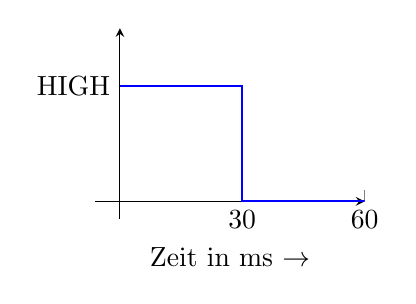
\begin{tikzpicture}
\begin{axis}[
width=5cm,
height=4cm,
x axis line style={-stealth},
y axis line style={-stealth},
yticklabels={HIGH},
xtick={30, 60},
ymax = 1.5,xmax=60,
axis lines*=center,
ytick={1},
xlabel={Zeit in ms $\rightarrow$},
xlabel near ticks,
ylabel near ticks]
\addplot+[thick,mark=none,const plot]
coordinates
{(0,1) (30,0) (60,0)};
\end{axis}
\end{tikzpicture}
\label{fig:s0impuls}
\caption{Idealisierter S0-Impuls}
\end{center}
\end{figure}

Die Anzahl der Impulse pro Zeiteinheit werden durch eine Wartezeit $ t_{S0} $ zwischen zwei Impulsen bestimmt. Hierzu müssen die Anzahl der Impulse pro Leistungsverbrauch $ n_{S0} $ und die Dauer einer Impulsphase $ t_p $ gegeben sein. Weiterhin müssen die Zeitdauer eines Simulationsschrittes in Millisekunden $ t_d $ bekannt sein und die verrichtete elektrische Arbeit $ Q_w $ berechnet werden. Die Berechnung von $ t_{S0} $ wird dann wie in Formel \ref{eq:sleeptime} durchgeführt.

\begin{equation}\label{eq:sleeptime}
t_{S0} = \frac{t_d}{n_{S0} Q_w - 2 t_p}
\end{equation}

\subsection{Kompilieren des Simulators}\label{simulatorcompile}
Um den Simulator zu kompilieren, gibt es einige Systemvoraussetzungen, die zunächst erfüllt werden müssen. Da die Applikation unter Linux (siehe Abschnitt \ref{os}) laufen soll, empfiehlt es sich, diese auch unter demselben Betriebssystem zu übersetzen. Zunächst wird ein C++-Compiler benötigt; in diesem Projekt wurde die \emph{GNU Compiler Collection} (kurz: GCC) verwendet. Diese ist unter Linux in der Regel in den Paketquellen zu finden. Alternativ kann man sie auch manuell installieren\footnote{https://gcc.gnu.org/install}. Anschließend werden noch die Programmbibliotheken \emph{Boost} und \emph{Wiring Pi} benötigt.
Sind alle Voraussetzungen erfüllt, lässt sich die Applikation mit dem Befehl \colorbox{lightgrey}{\lstinline[basicstyle=\ttfamily]|make|} kompilieren.

\subsection{Konfiguration des Simulators}

Viele der Werte, die in Abschnitt \ref{software_model} für das physikalische Modell verwendet werden, sind veränderlich. So unter anderem der Zeitschritt des Simulationsverfahren oder das Fassungsvermögen des zu simulierenden Eiswasserspeichers. Um dies zu ermöglichen, sollte die Applikation konfigurierbar sein, ohne diese stets neu kompilieren zu müssen. Um dies zu ermöglichen, werden sogenannte \emph{Initialisierungsdateien} (kurz: INI-Dateien) verwendet. Dies sind einfache Textdateien, deren Struktur aus Abschnitten, Eigenschaften und Werten besteht \cite{inifile}.
Zum Einlesen und Parsen der INI-Dateien wird die  \emph{Boost program\_options} Bibliothek verwendet.

Ein einfaches Beispiel einer Konfigurationsdatei ist in Listing \ref{lst:ini-example} zu sehen.

\begin{lstlisting}[frame=single, caption=INI-Datei Beispiel, label=lst:ini-example]
	[FooBar]
	prop = foobar
	prop.foo = foo
	prop.bar = bar
	[Baz]
	other = value
\end{lstlisting}

Die Konfigurationsmöglichkeiten des Simulators sind in Tabelle \ref{tab:simulatorconfig} aufgelistet, dabei sind sämtliche Zahlenwerte als \emph{Integer} anzugeben.

\begin{table}[H]
\centering
\begin{tabularx}{\textwidth}{|p{.3\textwidth}|p{.25\textwidth}|X|}
\hline
\textbf{Schlüssel} & \textbf{Mögliche Werte} & \textbf{Beschreibung} \\ \hline
controlserver.port & 1024 < port < 65535 & Port des Steuer-Servers \\ \hline
controlserver.secret.token & beliebig & Geheimer Schlüssel \\ \hline
milk.temp.target & > 0 & Zieltemperatur der Milch \\ \hline
milk.temp.input & > 0 & Eingangstemperatur der Milch \\ \hline
simulator.time.step & > 0 & Zeitschritt in Minuten \\ \hline
simulator.log.level & >= 10 für \emph{ERROR} & Log-Level des Simulators \\
 & >= 20 für \emph{WARN} & \\ 
 & >= 30 für \emph{INFO} & \\
 & >= 40 für \emph{DEBUG} & \\ 
 & >= 50 für \emph{TRACE} & \\ \hline
simulator.debug & true/false & Falls true, wird der Zeitschritt \\
 & & auf 10 Sekunden abgesenkt \\ \hline
snull.pin & S. Abschnitt \ref{gpio} & Pin für den Ausgang zur S0-Schnittstelle \\ \hline
snull.watt.per.pulse & > 0 & Anzahl der Pulse pro Watt \\ \hline
snull.watt.per.load & > 0 & Leistung beim Laden \\ \hline
snull.watt.per.cool & > 0 & Leistung beim Kühlen \\ \hline
reservoir.capacity & > 0 & Kapazität des Speichers \\ \hline
reservoir.loadingtime & > 0 & Ladezeit in Stunden \\ \hline
reservoir.pumps.flow & > 0 & Volumenstrom der Pumpen in l/min \\ \hline
\end{tabularx}
\caption{Konfiguration des Simulators}
\label{tab:simulatorconfig}
\end{table}

\section{Steuer-Client}\label{steuerclient}
Um den im vorherigen Abschnitt vorgestellten Steuer-Server einfach und sicher bedienen zu können, wurde im Rahmen dieses Projektes der \emph{Steuer-Client} entwickelt. Dies ist eine einfache C++-Applikation, die unabhängig vom Simulator gestartet und bedient werden kann. Dabei ist es möglich, dass Simulator und Steuer-Client auf physisch getrennten Maschinen laufen, da diese über TCP/IP miteinander kommunizieren. Dies wird bereits durch den Raspberry PI und das darauf laufende Betriebssystem sichergestellt (siehe Kapitel \ref{raspi}).

\subsection{Konfiguration des Steuer-Clients}
Auch der Steuer-Client ist über eine mitgelieferte INI-Datei konfigurierbar. Hierzu wird ebenfalls die \emph{Boost program\_options} Bibliothek verwendet.
Tabelle \ref{tab:clientconfig} zeigt die Konfigurationsmöglichkeiten des Steuer-Clients.

\begin{table}[h]
\centering
\begin{tabularx}{\textwidth}{|p{.3\textwidth}|p{.25\textwidth}|X|}
\hline
\textbf{Schlüssel} & \textbf{Mögliche Werte} & \textbf{Beschreibung} \\ \hline
server.host & beliebig & Hostname bzw. IP des Rechners, auf dem der Simulator läuft \\ \hline
server.port & 1024 < port < 65535 & Port des Rechners, auf dem der Simulator läuft \\ \hline
server.secret.token & beliebig & Geheimer Schlüssel des Servers \\ \hline
\end{tabularx}
\caption{Konfiguration des Steuer-Clients}
\label{tab:clientconfig}
\end{table}

\subsection{Kompilieren des Steuer-Clients}
Der Steuer-Client lässt sich nahezu analog zum Simulator kompilieren (siehe Abschnitt \ref{simulatorcompile}). Einzig die \emph{Wiring Pi} Bibliothek wird nicht benötigt. Wurden alle Voraussetzungen für den Simulator bereits geschaffen, so lässt sich der Steuer-Client ebenfalls mit dem Befehl \colorbox{lightgrey}{\lstinline[basicstyle=\ttfamily]|make|} kompilieren.